\documentclass[letterpaper, 12pt]{article}

% --- Package imports ---
\bibliographystyle{plain}
% Extended set of colors
\usepackage[dvipsnames]{xcolor}

\usepackage{
  amsmath, amsthm, amssymb, mathtools, dsfont, units,          % Math typesetting
  graphicx, wrapfig, subfig, float,                            % Figures and graphics formatting
  listings, color, inconsolata, pythonhighlight,               % Code formatting
  fancyhdr, sectsty, hyperref, enumerate, enumitem, framed }   % Headers/footers, section fonts, links, lists

% lipsum is just for generating placeholder text and can be removed
\usepackage{hyperref, lipsum} 

% --- Fonts ---

\usepackage{newpxtext, newpxmath, inconsolata}

% --- Page layout settings ---

% Set page margins
\usepackage[left=1.35in, right=1.35in, top=1.0in, bottom=.9in, headsep=.2in, footskip=0.35in]{geometry}

% Anchor footnotes to the bottom of the page
\usepackage[bottom]{footmisc}

% Set line spacing
\renewcommand{\baselinestretch}{1.2}

% Set spacing between paragraphs
\setlength{\parskip}{1.3mm}

% Allow multi-line equations to break onto the next page
\allowdisplaybreaks

% --- Page formatting settings ---

% Set image captions to be italicized
\usepackage[font={it,footnotesize}]{caption}

% Set link colors for labeled items (blue), citations (red), URLs (orange)
\hypersetup{colorlinks=true, linkcolor=RoyalBlue, citecolor=RedOrange, urlcolor=ForestGreen}

% Set font size for section titles (\large) and subtitles (\normalsize) 
\usepackage{titlesec}
\titleformat{\section}{\large\bfseries}{{\fontsize{19}{19}\selectfont\textreferencemark}\;\; }{0em}{}
\titleformat{\subsection}{\normalsize\bfseries\selectfont}{\thesubsection\;\;\;}{0em}{}

% Enumerated/bulleted lists: make numbers/bullets flush left
%\setlist[enumerate]{wide=2pt, leftmargin=16pt, labelwidth=0pt}
\setlist[itemize]{wide=0pt, leftmargin=16pt, labelwidth=10pt, align=left}

% --- Table of contents settings ---

\usepackage[subfigure]{tocloft}

% Reduce spacing between sections in table of contents
\setlength{\cftbeforesecskip}{.9ex}

% Remove indentation for sections
\cftsetindents{section}{0em}{0em}

% Set font size (\large) for table of contents title
\renewcommand{\cfttoctitlefont}{\large\bfseries}

% Remove numbers/bullets from section titles in table of contents
\makeatletter
\renewcommand{\cftsecpresnum}{\begin{lrbox}{\@tempboxa}}
\renewcommand{\cftsecaftersnum}{\end{lrbox}}
\makeatother

% --- Set path for images ---

\graphicspath{{Images/}{../Images/}}

% --- Math/Statistics commands ---

% Add a reference number to a single line of a multi-line equation
% Usage: "\numberthis\label{labelNameHere}" in an align or gather environment
\newcommand\numberthis{\addtocounter{equation}{1}\tag{\theequation}}

% Shortcut for bold text in math mode, e.g. $\b{X}$
\let\b\mathbf

% Shortcut for bold Greek letters, e.g. $\bg{\beta}$
\let\bg\boldsymbol

% Shortcut for calligraphic script, e.g. %\mc{M}$
\let\mc\mathcal

% \mathscr{(letter here)} is sometimes used to denote vector spaces
\usepackage[mathscr]{euscript}

% Convergence: right arrow with optional text on top
% E.g. $\converge[p]$ for converges in probability
\newcommand{\converge}[1][]{\xrightarrow{#1}}

% Weak convergence: harpoon symbol with optional text on top
% E.g. $\wconverge[n\to\infty]$
\newcommand{\wconverge}[1][]{\stackrel{#1}{\rightharpoonup}}

% Equality: equals sign with optional text on top
% E.g. $X \equals[d] Y$ for equality in distribution
\newcommand{\equals}[1][]{\stackrel{\smash{#1}}{=}}

% Normal distribution: arguments are the mean and variance
% E.g. $\normal{\mu}{\sigma}$
\newcommand{\normal}[2]{\mathcal{N}\left(#1,#2\right)}

% Uniform distribution: arguments are the left and right endpoints
% E.g. $\unif{0}{1}$
\newcommand{\unif}[2]{\text{Uniform}(#1,#2)}

% Independent and identically distributed random variables
% E.g. $ X_1,...,X_n \iid \normal{0}{1}$
\newcommand{\iid}{\stackrel{\smash{\text{iid}}}{\sim}}

% Sequences (this shortcut is mostly to reduce finger strain for small hands)
% E.g. to write $\{A_n\}_{n\geq 1}$, do $\bk{A_n}{n\geq 1}$
\newcommand{\bk}[2]{\{#1\}_{#2}}

% Math mode symbols for common sets and spaces. Example usage: $\R$
\newcommand{\R}{\mathbb{R}}	% Real numbers
\newcommand{\C}{\mathbb{C}}	% Complex numbers
\newcommand{\Q}{\mathbb{Q}}	% Rational numbers
\newcommand{\Z}{\mathbb{Z}}	% Integers
\newcommand{\N}{\mathbb{N}}	% Natural numbers
\newcommand{\F}{\mathcal{F}}	% Calligraphic F for a sigma algebra
\newcommand{\El}{\mathcal{L}}	% Calligraphic L, e.g. for L^p spaces

% Math mode symbols for probability
\newcommand{\pr}{\mathbb{P}}	% Probability measure
\newcommand{\E}{\mathbb{E}}	% Expectation, e.g. $\E(X)$
\newcommand{\var}{\text{Var}}	% Variance, e.g. $\var(X)$
\newcommand{\cov}{\text{Cov}}	% Covariance, e.g. $\cov(X,Y)$
\newcommand{\corr}{\text{Corr}}	% Correlation, e.g. $\corr(X,Y)$
\newcommand{\B}{\mathcal{B}}	% Borel sigma-algebra

% Other miscellaneous symbols
\newcommand{\tth}{\text{th}}	% Non-italicized 'th', e.g. $n^\tth$
\newcommand{\Oh}{\mathcal{O}}	% Big-O notation, e.g. $\O(n)$
\newcommand{\1}{\mathds{1}}	% Indicator function, e.g. $\1_A$

% Algebra operations
\newcommand{\inner}[2]{\langle #1, #2 \rangle}
\newcommand{\norm}[1]{\| #1 \|}

% Additional commands for math mode
\DeclareMathOperator*{\argmax}{argmax}		% Argmax, e.g. $\argmax_{x\in[0,1]} f(x)$
\DeclareMathOperator*{\argmin}{argmin}		% Argmin, e.g. $\argmin_{x\in[0,1]} f(x)$
\DeclareMathOperator*{\spann}{Span}		% Span, e.g. $\spann\{X_1,...,X_n\}$
\DeclareMathOperator*{\bias}{Bias}		% Bias, e.g. $\bias(\hat\theta)$
\DeclareMathOperator*{\ran}{ran}			% Range of an operator, e.g. $\ran(T) 
\DeclareMathOperator*{\dv}{d\!}			% Non-italicized 'with respect to', e.g. $\int f(x) \dv x$
\DeclareMathOperator*{\diag}{diag}		% Diagonal of a matrix, e.g. $\diag(M)$
\DeclareMathOperator*{\trace}{trace}		% Trace of a matrix, e.g. $\trace(M)$
\DeclareMathOperator*{\supp}{supp}		% Support of a function, e.g., $\supp(f)$

% Numbered theorem, lemma, etc. settings - e.g., a definition, lemma, and theorem appearing in that 
% order in Lecture 2 will be numbered Definition 2.1, Lemma 2.2, Theorem 2.3. 
% Example usage: \begin{theorem}[Name of theorem] Theorem statement \end{theorem}
\theoremstyle{definition}
\newtheorem{theorem}{Theorem}[section]
\newtheorem{proposition}[theorem]{Proposition}
\newtheorem{lemma}[theorem]{Lemma}
\newtheorem{corollary}[theorem]{Corollary}
\newtheorem{definition}[theorem]{Definition}
\newtheorem{example}[theorem]{Example}
\newtheorem{remark}[theorem]{Remark}

% Un-numbered theorem, lemma, etc. settings
% Example usage: \begin{lemma*}[Name of lemma] Lemma statement \end{lemma*}
\newtheorem*{theorem*}{Theorem}
\newtheorem*{proposition*}{Proposition}
\newtheorem*{lemma*}{Lemma}
\newtheorem*{corollary*}{Corollary}
\newtheorem*{definition*}{Definition}
\newtheorem*{example*}{Example}
\newtheorem*{remark*}{Remark}
\newtheorem*{claim}{Claim}

% --- Left/right header text (to appear on every page) ---

% Do not include a line under header or above footer
\pagestyle{fancy}
\renewcommand{\footrulewidth}{0pt}
\renewcommand{\headrulewidth}{0pt}

% Right header text: Lecture number and title
\renewcommand{\sectionmark}[1]{\markright{#1} }
\fancyhead[R]{\small\textit{\nouppercase{\rightmark}}}

% Left header text: Short course title, hyperlinked to table of contents
\fancyhead[L]{\hyperref[sec:contents]{\small Short title of document}}

% --- Document starts here ---

\begin{document}

% --- Main title and subtitle ---

\title{Curvature and Vector Fields \\[1em]
\normalsize Lecture Notes of Loring W. Tu \cite{tu2010introduction}}

% --- Author and date of last update ---

\author{\normalsize Zhenhao Huang}
\date{\normalsize\vspace{-1ex} Last updated: \today}

% --- Add title and table of contents ---

\maketitle
\tableofcontents\label{sec:contents}

% --- Main content: import lectures as subfiles ---

% TeX root = main.tex

% First argument to \section is the title that will go in the table of contents. Second argument is the title that will be printed on the page.
\section[Lecture 1--{Riemannian manifold}]{1. Riemannian manifold}
A Riemannian manifold is a manifold endowed with a Riemannian metric.
The Riemannian metric is a smoothly varying inner product on tangent space at each point.
This section first recall the definition of inner product, then we prove the existence
of a Riemannian metric on any smooth manifolds.
\subsection{Inner Products on a Vector Space}
The $\textbf{Euclidean inner product}$ on $\mathbb{R}^n$ is defined by
\begin{align}
    \inner{u}{v}=\sum_{1}^{n}u^i v^i,
\end{align}
and the length of a vector is
\begin{align}
    \norm{u}=\sqrt{\inner{u}{u}},
\end{align}
the \textbf{angle} $\boldsymbol{\theta}$ between two vectors is
\begin{align}
    \cos \theta = \frac{\inner{u}{v}}{\norm{u}\norm{v}},
\end{align}
the \textbf{arc length} of a curve $c(t) \in \mathbb{R}^n, a \leq t \leq b$ is 
\begin{align}
    s = \int_{a}^{b} \norm{c'(t)} dt
\end{align}

\begin{definition}
    An inner product in a real vector space $V$ is a postive-definite,
    bilinear and symmetric map: $\inner{\cdot}{\cdot}: 
    V \times V \rightarrow \mathbb{R}$ 
    so that for $u,v,w \in V$ and $a,b\in \mathbb{R}$, satisfies
    \begin{enumerate}[label= (\roman*)]
        \item \textbf{Postive-definiteness} $\inner{v}{v}=0$ iff. $v=0$
        \item \textbf{Symmetry} $\inner{u}{v}=\inner{v}{u}$
        \item \textbf{Bilinear} $\inner{au+bv}{w}=a\inner{u}{w}+b\inner{v}{w}$
    \end{enumerate}
\label{def. inner prodcut}
\end{definition}

\begin{proposition}
    If $W$ is a subspace of $V$, then the restriction
    \begin{align}
        \inner{}{}_W:=\inner{}{}|_{W\times W}: W \times W \rightarrow \mathbb{R},
    \end{align}
    of an inner product
    $\inner{}{}$ on $V$ is also an innver prodcut.
\end{proposition}
\begin{proof}
    The subspace construction preserves the properites 
    in Definition~\ref{def. inner prodcut}.
\end{proof}

\begin{proposition}
    The \textbf{nonnegative linear combinition} of inner products $\inner{}{}_i$
     on $V$: $\inner{}{}:=\sum_{i=1}^{r}a_i\inner{}{}_i, a_i \geq 0$ is again an 
     inner product on $V$.
\label{prop. nonneg combinition of metrics}
\end{proposition}
\begin{proof}
    The \textbf{nonnegativity} of $a_i$ preserves condition $(i)$ 
    in Definition~\ref{def. inner prodcut}, the linearity makes condition $(ii),(iii)$ hold.
\end{proof}

\subsection{Representations of Inner Products by Symmetric Matrices}
Let $e_1,\dots, e_n$ be the basis of vector space $V$, 
each vector $x \in V$ can be represented as a column vector
\begin{equation}
    x=\sum_{i=1}^{n}x^i e_i \leftrightarrow \vx=\left[\begin{array}{c}
        x^1 \\
        \vdots \\
        x^n
    \end{array}\right].
\end{equation}
Let $\mA$ be an $n\times n$ matrix whose entries $a_{ij}=\inner{e_i}{e_j}$, 
the matrix form of an inner product on $V$ is
\begin{equation}
    \inner{x}{y}=\sum_{ij}x^i y^j \inner{e_i}{e_j} = \vx^\top \mA \vy.
\end{equation}
We find that, once a basis of $V$ is chosen, the inner product on $V$
determines a postive-definite symmetric matrix. Conversely, an $n \times n$
postive-definite symmetric matrix with a basis of $V$ determines an inner product 
on $V$

It follows that there is an one-to-one correspondence
\begin{align}
    \left\{
    \begin{array}{c}
        \text{inner product on a $n$-dimensional} \\
        \text{vector space}
    \end{array}
\right\}
\leftrightarrow
\left\{
    \begin{array}{c}
        \text{An $n \times n$ postive-definite} \\
        \text{symmetric matrix}
    \end{array}
\right\}.
\end{align}
Let a basis of dual space $V^\vee:=\Hom{V, \sR}$ be $\alpha^1,\dots,\alpha^n$ w.r.t.
the basis $e_1,\dots,e_n$ of $V$, an inner product $\inner{}{}$ of $x,y\in V$ is
\begin{align}
    \inner{x}{y}&=\sum_{i,j} a_{ij} x^i y^j=\sum_{i,j} a_{ij} \alpha^i(x) \alpha^j(y) \nonumber \\
    &=\sum_{i,j} a_{ij} \alpha^i \otimes \alpha^j (x,y) \nonumber
\end{align}
In terms of tensor product, an inner product on $V$ may be written as
\begin{align}
    \inner{}{} = \sum_{ij}a_{ij} \alpha^i \otimes \alpha^j
\end{align}
\subsection{Riemannian Metrics}
\begin{definition}
    \label{def. Riemannian metric}
    A \textbf{Riemannian metric} is an inner product \textbf{assignment} 
    to each $p \in M$ of an inner product $\inner{}{}_p$ on the tangent space $T_p M$.
    This assignment should be $C^\infty$ in the following sense: 
    if $p \mapsto \inner{X_p}{Y_p}_p$ is a $C^\infty$ function for any $C^\infty$ 
    vector fields $X,Y$. A \textbf{Riemannian manifold} is a pair $(M, \inner{}{})$, 
    which consists of a $C^\infty$ manifold $M$ together with 
    a Riemannian metric on $M$.
\end{definition}
\begin{example}
    Since the tangent space at a point in Euclidean space $\sR^n$ 
    is isomorphic to $\sR^n$, the Euclidean inner product induces a Riemannian metric 
    on $\sR^n$ called the \textbf{Euclidean metric}.
\end{example}
\begin{example}
    A surface $M$ in $\sR^3$ is a $2$-dimensional regular submanifold of $\sR^3$, 
    the tangent space at $p$ is a subspace of $T_p\sR^3$, so the surface $M$ inherits 
    a Riemannian metric from the Euclidean metric by restriction $\inner{}{}_M$.
\end{example}
\begin{definition}
    A $C^\infty$ map $F: (N, \inner{}{}') \rightarrow (M, \inner{}{})$ of 
    Riemannian manifolds is said to be \textbf{metric-preserving} if 
    \begin{equation}
        \inner{u}{v}'_p = \inner{F_*u}{F_*v}_{F(p)}
        \label{eq. metric-preserving}
    \end{equation}
    for all point $p \in N$ and tangent vectors $u,v \in T_p N$. 
    An \textbf{isometry}
    is a metric-preserving diffeomorphism.
\end{definition}
For a Riemannian manifold $(M, \inner{}{})$, if there is a diffeomorphism that maps some
manifolds $N$ to $M$, the induced metric $\inner{}{}'$ on $N$
 can be defined by (\ref{eq. metric-preserving}).
\begin{example}[Metric-preserving but not an isometry]
    Let $N$ and $M$ be the unit circle in $\mathbb{C}$. 
    Define $F: N \rightarrow M$ a \textbf{2-sheeted covering space map} 
    (for any $w \in M$, $F^{-1}(w)$ contains $2$ points in $N$), 
    by $F(z)=z^2$. Given $M$
    any Riemannian metric $\inner{}{}$, and define the induced metric 
    on $N$ is (\ref{eq. metric-preserving}),
    The map $F$ is metric-preserving 
    but not an isometry because $F$ is not a diffeomorphism (not inject).
\end{example}
\begin{example}[Topological equivalant Riemannian manifolds may not isometric]
    
\end{example}

\begin{figure}[htp]
    \centering
    \subfloat[]{
        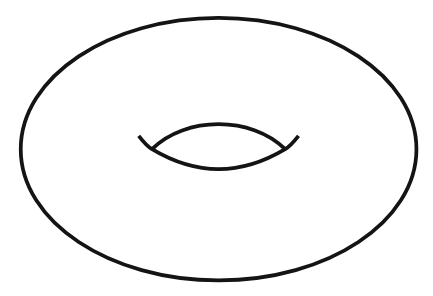
\includegraphics[width=0.3\textwidth]{../Lectures/Figures/torus_1.png}
    }
    \subfloat[]{
        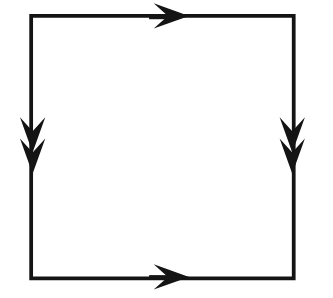
\includegraphics[width=0.3\textwidth]{../Lectures/Figures/torus_2.png}
    }
    \caption{Two Riemannian metrics on torus~\cite[p.~6]{tu2010introduction}.}
\end{figure}
\subsection{Existence of a Riemannian Metric}
The local diffeomorphism $\phi$ defines a Riemannian metric on 
a coordinate chart $(U, x^1,\dots, x^n)$ of $M$ that $x^i=r^i \circ \phi$, 
as
\begin{equation}
    \inner{X}{Y}=\sum_{ij}a^i b^i\inner{\partial_i}{\partial_j}
    =\sum_{ij}a^i b^i,
    \label{eq. induced inner}
\end{equation}
since $\phi_* \partial_j=\frac{\partial}{\partial r^j}$, the induced metric 
is the same as the Euclidean ones.

To obtain a Riemannian metric on $M$, we need to piece together the Riemannian 
metrics on all charts of an atlas of $M$. Here, we use the 
\textbf{partition of the unity} as the standard tools.
\begin{theorem}[Existence of a Riemannian metric]
    There exists a Riemannian metric on every manifold.
\end{theorem}
\begin{proof}
    Let $\{(U_\alpha, \phi_\alpha)\}_{\alpha \in A}$ an atlas of $M$. 
    We have a partition of unity $\{\rho_\alpha\}$ that subcoordinates to 
    open sets $\{U_\alpha\}$. 
    Let $\inner{}{}_\alpha$ the Riemannian metric on $U_\alpha$ as in (\ref{eq. induced inner}), 
    from Proposition~\ref{prop. nonneg combinition of metrics}, we define a metric
    on $T_pM$ at $p$ is 
    \begin{align}
        \inner{}{} = \sum_{\alpha\in A} \rho_\alpha \inner{}{}_\alpha.
        \label{eq. piece together metric}
    \end{align}
    Since $U_p$ intersects finite number of $U_\alpha$, (\ref{eq. piece together metric}) is
    a finite sum.
    Since $\rho_\alpha$ and $\inner{}{}_\alpha$ are both smooth, for any $C^\infty$
    vector fields $X, Y$,
    $\sum_{\alpha\in A} \rho_\alpha \inner{X}{Y}_\alpha$ 
    is a finite sum of smooth functions at arbitary $p$
     (By Definition~\ref{def. Riemannian metric}). 
     So $\sum_{\alpha\in A} \rho_\alpha \inner{}{}_\alpha$ is a Riemannian metric on $M$.
\end{proof}

\problemsection{Problems}
\begin{problem}
    Suppose $(M, \inner{}{})$ is a Riemannian manifold. Show that two $C^\infty$ vector fields
    $X,Y \in \mathfrak{X}(M)$ are equal if and only if $\inner{X}{Z}=\inner{Y}{Z}$ for all
    $C^\infty$ vector fields $Z\in\mathfrak{X}(M)$.
\end{problem}

% --- Bibliography ---

% Start a bibliography with one item.
% Citation example: "\cite{williams}".

\bibliography{reference}

% --- Document ends here ---

\end{document}
